% Figure: Wikipedia Multi-Agent Routing Architecture
% Shows user query → router → cached expert agents → synthesis

\begin{figure}[t]
\centering
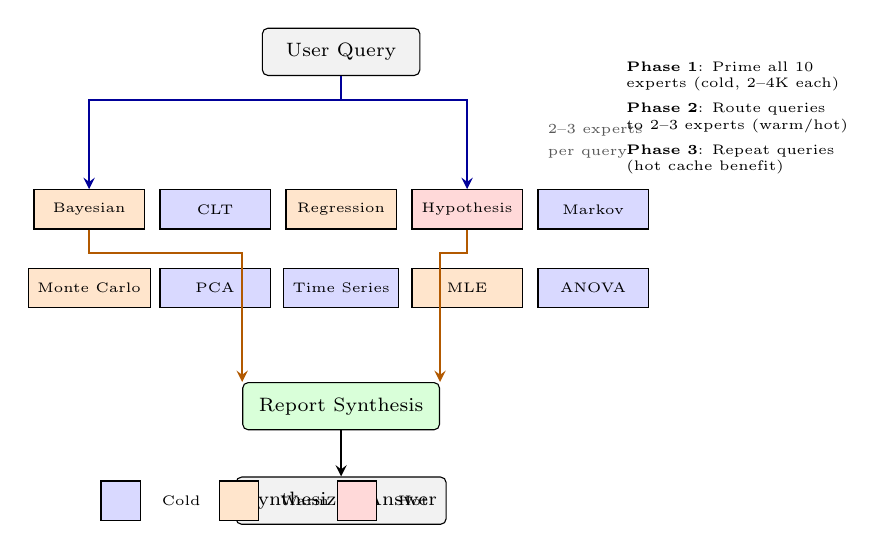
\begin{tikzpicture}[
    node distance=0.5cm,
    box/.style={rectangle, draw=black, rounded corners=2pt, minimum height=0.6cm, align=center, font=\scriptsize},
    expert/.style={rectangle, draw=black, minimum width=1.4cm, minimum height=0.5cm, align=center, font=\tiny},
    cold/.style={fill=blue!15},
    warm/.style={fill=orange!20},
    hot/.style={fill=red!15},
    arrow/.style={->, >=stealth, thick},
    label/.style={font=\tiny, text=gray!70!black}
]

% User query
\node[box, fill=gray!10, minimum width=2cm] (user) at (0, 3.5) {User Query};

% Expert agents grid (2 rows of 5)
\foreach \i/\name/\state in {
    0/Bayesian/warm,
    1/CLT/cold,
    2/Regression/warm,
    3/Hypothesis/hot,
    4/Markov/cold} {
    \node[expert, \state] (e\i) at (\i*1.6 - 3.2, 1.5) {\name};
}
\foreach \i/\name/\state in {
    5/Monte Carlo/warm,
    6/PCA/cold,
    7/Time Series/cold,
    8/MLE/warm,
    9/ANOVA/cold} {
    \pgfmathsetmacro{\x}{(\i-5)*1.6 - 3.2}
    \node[expert, \state] (e\i) at (\x, 0.5) {\name};
}

% Article cache indicators (small boxes below experts)
\foreach \i in {0,...,9} {
    \pgfmathsetmacro{\y}{ifthenelse(\i<5, 1.1, 0.1)}
    \pgfmathsetmacro{\x}{ifthenelse(\i<5, \i*1.6-3.2, (\i-5)*1.6-3.2)}
}

% Arrows from user to relevant experts (highlighted)
\draw[arrow, blue!60!black] (user.south) -- ++(0,-0.3) -| (e0.north);
\draw[arrow, blue!60!black] (user.south) -- ++(0,-0.3) -| (e3.north);

% Label: "2--3 experts per query"
\node[label, anchor=west] at (2.5, 2.5) {2--3 experts};
\node[label, anchor=west] at (2.5, 2.2) {per query};

% Synthesis agent
\node[box, fill=green!15, minimum width=2.5cm] (synth) at (0, -1.0) {Report Synthesis};

% Arrows from selected experts to synthesis
\draw[arrow, orange!70!black] (e0.south) -- ++(0,-0.3) -| (synth.north west);
\draw[arrow, orange!70!black] (e3.south) -- ++(0,-0.3) -| (synth.north east);

% Output
\node[box, fill=gray!10, minimum width=2cm] (out) at (0, -2.2) {Synthesized Answer};
\draw[arrow] (synth) -- (out);

% Phase annotations on right
\node[font=\tiny, align=left, anchor=north west] at (3.5, 3.5) {
    \textbf{Phase 1}: Prime all 10\\
    experts (cold, 2--4K each)\\[3pt]
    \textbf{Phase 2}: Route queries\\
    to 2--3 experts (warm/hot)\\[3pt]
    \textbf{Phase 3}: Repeat queries\\
    (hot cache benefit)
};

% Legend
\node[expert, cold, minimum width=0.5cm] at (-2.8, -2.2) {};
\node[font=\tiny, anchor=west] at (-2.4, -2.2) {Cold};
\node[expert, warm, minimum width=0.5cm] at (-1.3, -2.2) {};
\node[font=\tiny, anchor=west] at (-0.9, -2.2) {Warm};
\node[expert, hot, minimum width=0.5cm] at (0.2, -2.2) {};
\node[font=\tiny, anchor=west] at (0.6, -2.2) {Hot};

\end{tikzpicture}
\caption{Wikipedia multi-agent routing. Ten expert agents are primed with article content (cold prefill). Cross-topic queries route to 2--3 relevant experts whose caches are warm/hot from priming. A reporter agent synthesizes responses. Repeated queries to the same experts benefit from hot cache (projected 10--30$\times$ TTFT reduction vs cold).}
\label{fig:wikirouting}
\end{figure}
